\documentclass{article}
\usepackage[utf8]{inputenc}
\usepackage[T1]{fontenc}
\usepackage{graphicx}
\usepackage{hyperref}
\usepackage{geometry}
\geometry{margin=1in}

\title{DAMSEL}
\date{Encyclopaedia Britannica (1771)}

\begin{document}
\maketitle

\section*{Historical source}
\textbf{Entry ID:} \texttt{entry-damsel-1214} \\
\textbf{Volume ID:} 149979156 \\
\textbf{Character Count:} 553

\subsection*{Extracted Text}
DAMSEL, from the French \_damself or demasifons\_, an application ancestri given to all young people of eitherys, that were of endular or genest extraction, as the fons and daughters of princes, knights, and barons: thus we read of Daniel Prisin DaudiL Louis le Gros, David Richard spruce (My Wales.

From the folos of Kings this appellation ftp piled to theife of great locals and barons, and a length to think of gestionome who were not yet lengths.

At present damful is applied to all meals or girls not yet material, provided by be not of the vulgar.



\section*{Source record}
\begin{itemize}
\item \textbf{Dataset:} \texttt{NationalLibraryOfScotland/encyclopaedia\_britannica\_illustrated}
\item \textbf{Dataset Revision:} \texttt{309f765b1ecc83e0a7f7762e44b4a927a7555443}
\item \textbf{Page ID:} \texttt{britannica:309f765b1ecc83e0a7f7762e44b4a927a7555443:train:1214} \\
  \textbf{Filename:} \texttt{page-1214-17d180a99e0a.jpg} \\
  \textbf{Row Index:} 1214 \\
  \textbf{SHA256:} \texttt{17d180a99e0a4854...}
\end{itemize}

\begin{figure}[h]
\centering
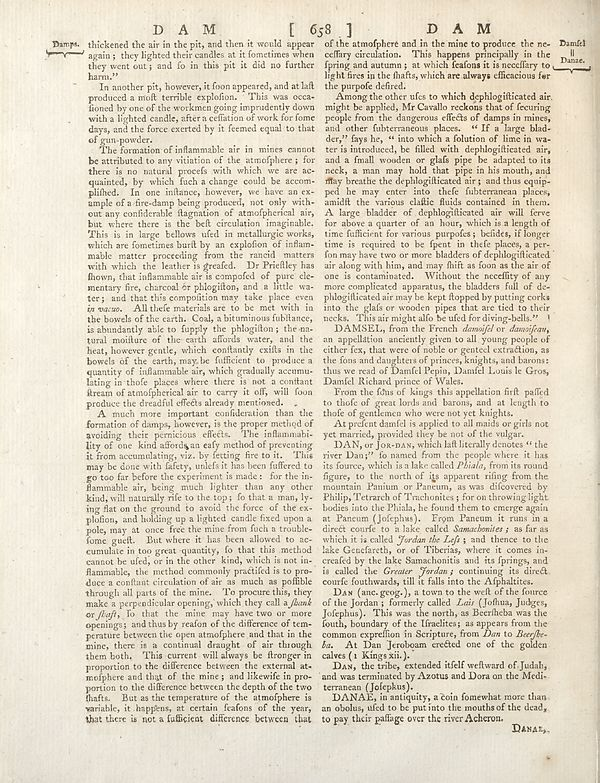
\includegraphics[width=0.85\textwidth]{../scans/page-1214-17d180a99e0a.jpg}
\caption*{Source scan: \texttt{page-1214-17d180a99e0a.jpg}}
\end{figure}

\end{document}
